% ============================================================
%  Aligning Small LLMs with GRPO for Strict JSON Generation
%  Beamer presentation — Metropolis theme + Fira Sans
%  Compile with: pdflatex main.tex
% ============================================================

\documentclass[10pt, aspectratio=169]{beamer}

% ── Theme ────────────────────────────────────────────────
\usetheme{metropolis}
\usepackage{appendixnumberbeamer}

% ── Packages ─────────────────────────────────────────────
\usepackage{booktabs}
\usepackage{tabularx}
\usepackage{array}
\usepackage{xcolor}
\usepackage[T1]{fontenc}
\usepackage[sfdefault,scaled=.9]{FiraSans}
\usepackage[lining,scaled=.88]{FiraMono}
\usepackage{graphicx}
\usepackage{microtype}
\usepackage{tikz}
\usetikzlibrary{arrows.meta, positioning, calc}

% ── Colour palette ───────────────────────────────────────
\definecolor{navy}{HTML}{1B2A4A}
\definecolor{sky}{HTML}{0EA5E9}
\definecolor{offwhite}{HTML}{F8FAFC}

% ── Metropolis colour overrides ──────────────────────────
\setbeamercolor{normal text}      {fg=navy,   bg=white}
\setbeamercolor{frametitle}       {bg=navy,   fg=white}
\setbeamercolor{title separator}  {fg=sky}
\setbeamercolor{progress bar}     {fg=sky,    bg=navy!40}
\setbeamercolor{alerted text}     {fg=sky}
\setbeamercolor{block title}      {bg=navy!10, fg=navy}
\setbeamercolor{block body}       {bg=navy!5}
\setbeamercolor{title}            {fg=navy}
\setbeamercolor{subtitle}         {fg=navy}
\setbeamercolor{author}           {fg=navy}
\setbeamercolor{date}             {fg=navy}

% ── Metropolis options ───────────────────────────────────
\metroset{
  titleformat  = regular,
  progressbar  = frametitle,
  block        = fill,
  sectionpage  = none,
  numbering    = fraction,
}

% ── Metadata ─────────────────────────────────────────────
\title{Aligning Small LLMs with GRPO\\[0.25em]for Strict JSON Generation}
\subtitle{Rule-Based Reward Optimization for Schema-Conformant Output}
\author{Giuseppe Bellamacina}
\date{2026}

% ============================================================
\begin{document}

% ── Slide 1 · Title ─────────────────────────────────────
{
  \setbeamercolor{background canvas}{bg=offwhite}
  \maketitle
}

% ── Slide 2 · Problem & Objective ───────────────────────
\begin{frame}{Problem \& Objective}
  \begin{itemize}
    \setlength\itemsep{0.75em}
    \item Small LLMs ($<$2B parameters) frequently fail to produce valid,
          schema-conformant JSON
    \item Common errors: unclosed brackets, type violations, conversational filler
    \item \textbf{Goal:} use GRPO with rule-based rewards to reach
          $>$90\% Pass@1 on strict JSON
    \item No neural reward model $\rightarrow$
          dense, \alert{deterministic}, interpretable signal
  \end{itemize}
\end{frame}

% ── Slide 3 · Models & Setup ────────────────────────────
\begin{frame}{Models \& Hardware Configuration}
  \begin{columns}[T]
    \begin{column}{0.54\textwidth}
      \renewcommand{\arraystretch}{1.35}
      \begin{tabular}{@{}lrl@{}}
        \toprule
        \textbf{Model}         & \textbf{Params} & \textbf{Architecture} \\
        \midrule
        SmolLM2-135M-Instruct  & 135M & LLaMA-like \\
        SmolLM2-360M-Instruct  & 360M & LLaMA-like \\
        Qwen2.5-0.5B-Instruct  & 0.5B & Qwen2.5 \\
        TinyLlama-1.1B-Chat    & 1.1B & LLaMA 2 \\
        Gemma-2-2B-it          &   2B & Gemma 2 \\
        \bottomrule
      \end{tabular}
    \end{column}
    \begin{column}{0.43\textwidth}
      \vspace{0.4em}
      \begin{itemize}
        \setlength\itemsep{0.6em}
        \item 4-bit NF4 quantization
        \item LoRA \quad $r{=}16$,\; $\alpha{=}32$
        \item 1$\times$ NVIDIA L40S
        \item 2\,500 training steps / model
      \end{itemize}
    \end{column}
  \end{columns}
\end{frame}

% ── Slide 4 · GRPO Algorithm ────────────────────────────
\begin{frame}{Group Relative Policy Optimization (GRPO)}
  \centering
  \resizebox{\textwidth}{!}{%
  \begin{tikzpicture}[
    node distance=0cm and 0.65cm,
    box/.style={
      rectangle, rounded corners=5pt,
      minimum width=3.1cm, minimum height=1.55cm,
      text centered, inner sep=6pt, text width=3.0cm,
      draw=navy, thick
    },
    sbox/.style={
      rectangle, rounded corners=3pt,
      minimum width=1.55cm, minimum height=0.65cm,
      text centered, inner sep=3pt, text width=1.5cm,
      draw=sky!55, fill=sky!7, thick, font=\scriptsize
    },
    arr/.style={-{Stealth[length=7pt]}, thick, color=navy},
    sarr/.style={-{Stealth[length=5pt]}, thick, color=sky!70},
  ]
    % ── Main pipeline nodes ──────────────────────────────
    \node[box, fill=sky!10] (p)
      {\small\textbf{Prompt} $x$\\[4pt]
       \scriptsize sampled from dataset\\
       difficulty $d\in\{S,M,H\}$};

    \node[box, fill=navy!8, right=0.65cm of p] (g)
      {\small\textbf{Sample} $G{=}8$\\[4pt]
       \scriptsize $y_1,\dots,y_8\sim\pi_\theta(\cdot|x)$\\
       temp $T\in[0.6,\,0.8]$};

    \node[box, fill=sky!30, right=0.65cm of g] (r)
      {\small\textbf{Score} $r_i$\\[4pt]
       \scriptsize $r_i=\sum\nolimits_k w_k\,r_k(y_i)$\\
       7 additive components};

    \node[box, fill=navy!13, right=0.65cm of r] (a)
      {\small\textbf{Advantage} $\hat{A}_i$\\[4pt]
       \scriptsize $\hat{A}_i=\dfrac{r_i-\bar{r}_G}{\sigma_{r_G}}$\\[2pt]
       group-relative norm.};

    \node[box, fill=sky!18, right=0.65cm of a] (u)
      {\small\textbf{Update} $\pi_\theta$\\[4pt]
       \scriptsize $\mathcal{L}=\sum_i\hat{A}_i\log\pi_\theta(y_i|x)$\\
       $-\,\beta\,D_{\mathrm{KL}}$,\quad$\beta{=}0.04$};

    % ── Arrow labels ─────────────────────────────────────
    \draw[arr] (p) -- node[above,font=\tiny,color=navy]{prompt} (g);
    \draw[arr] (g) -- node[above,font=\tiny,color=navy]{$G$ completions} (r);
    \draw[arr] (r) -- node[above,font=\tiny,color=navy]{$\{r_i\}$} (a);
    \draw[arr] (a) -- node[above,font=\tiny,color=navy]{$\{\hat{A}_i\}$} (u);

    % ── Feedback loop ─────────────────────────────────────
    \draw[arr, dashed, color=navy!70, rounded corners=8pt]
      (u.south) -- ++(0,-0.75)
      -- node[below, font=\tiny, color=navy, pos=0.5]
         {updated $\pi_\theta$ becomes the new reference policy}
      ($(p.south)+(0,-0.75)$) -- (p.south);

    % ── Reward component sub-boxes (below Score node) ─────
    \node[sbox, below=1.15cm of r, xshift=-3.7cm] (c1) {format\\$w{=}0.20$};
    \node[sbox, right=0.12cm of c1]               (c2) {validity\\$w{=}0.25$};
    \node[sbox, right=0.12cm of c2]               (c3) {schema\\$w{=}0.25$};
    \node[sbox, right=0.12cm of c3]               (c4) {trunc.\\$w{=}0.10$};
    \node[sbox, right=0.12cm of c4]               (c5) {repet.\\$w{=}0.10$};
    \node[sbox, right=0.12cm of c5]               (c6) {strict.\\$w{=}0.10$};

    % horizontal collector bar + single arrow to Score node
    \coordinate (left)  at (c1.north west);
    \coordinate (right) at (c6.north east);
    \coordinate (mid)   at ($(left)!0.5!(right)$);
    \draw[sarr, rounded corners=2pt]
      (left) -- (right)
      (mid)  -- (r.south);

  \end{tikzpicture}}

  \vspace{0.3em}
  \raggedright\footnotesize
  \begin{itemize}
    \setlength\itemsep{0.38em}
    \item No neural reward model — scoring is \alert{deterministic} and \alert{interpretable}
    \item Additive composition prevents \alert{zero-advantage collapse}: gradient is always non-zero
    \item KL penalty ($\beta{=}0.04$) keeps $\pi_\theta$ close to the reference policy
  \end{itemize}
\end{frame}

% ── Slide 5 · Reward Functions ──────────────────────────
\begin{frame}{Rule-Based Reward System}
  \centering
  \scriptsize
  \renewcommand{\arraystretch}{1.32}
  \setlength\tabcolsep{4pt}
  \begin{tabularx}{0.99\linewidth}{@{}l@{\;}c@{\;}c@{\;}c@{\;}X@{}}
    \toprule
    \textbf{Component} & \textbf{Range} & \textbf{Think $w$} & \textbf{NoThink $w$} & \textbf{What it measures} \\
    \midrule
    \texttt{format}     & $[0,1]$      & 0.10 & 0.20 & \texttt{```json```} fence: 1.0 $\mid$ generic fence: 0.5 $\mid$ none: 0.0 \\
    \texttt{validity}   & $[0,1]$      & 0.15 & 0.25 & JSON parseability; partial credit by error position (0.20–0.70 if invalid) \\
    \texttt{schema}     & $[0,1]$      & 0.20 & 0.25 & Keys, types, nesting depth, required fields; 1.0 if valid but unconstrained \\
    \texttt{reasoning}  & $[-0.5,1]$   & 0.25 & \alert{0.0}  & \texttt{<think>} block quality: penalises missing/copied placeholder \\
    \texttt{truncation} & $[-1,1]$     & 0.10 & 0.10 & Unclosed braces / unterminated strings / trailing commas \\
    \texttt{repetition} & $[-1,1]$     & 0.10 & 0.10 & Token loops, repeated lines, duplicate blocks \\
    \texttt{strictness} & $[-1,1]$     & 0.10 & 0.10 & Extra text outside JSON $>$50\% of output \\
    \bottomrule
  \end{tabularx}
  \vspace{0.4em}

  \small\textit{Additive composition — no hard gating, gradient is always non-zero.}
\end{frame}

% ── Slide 5b · Reward Breakdown (SmolLM2-135M) ──────────
\begin{frame}{Reward Breakdown — SmolLM2-135M}
  \centering
  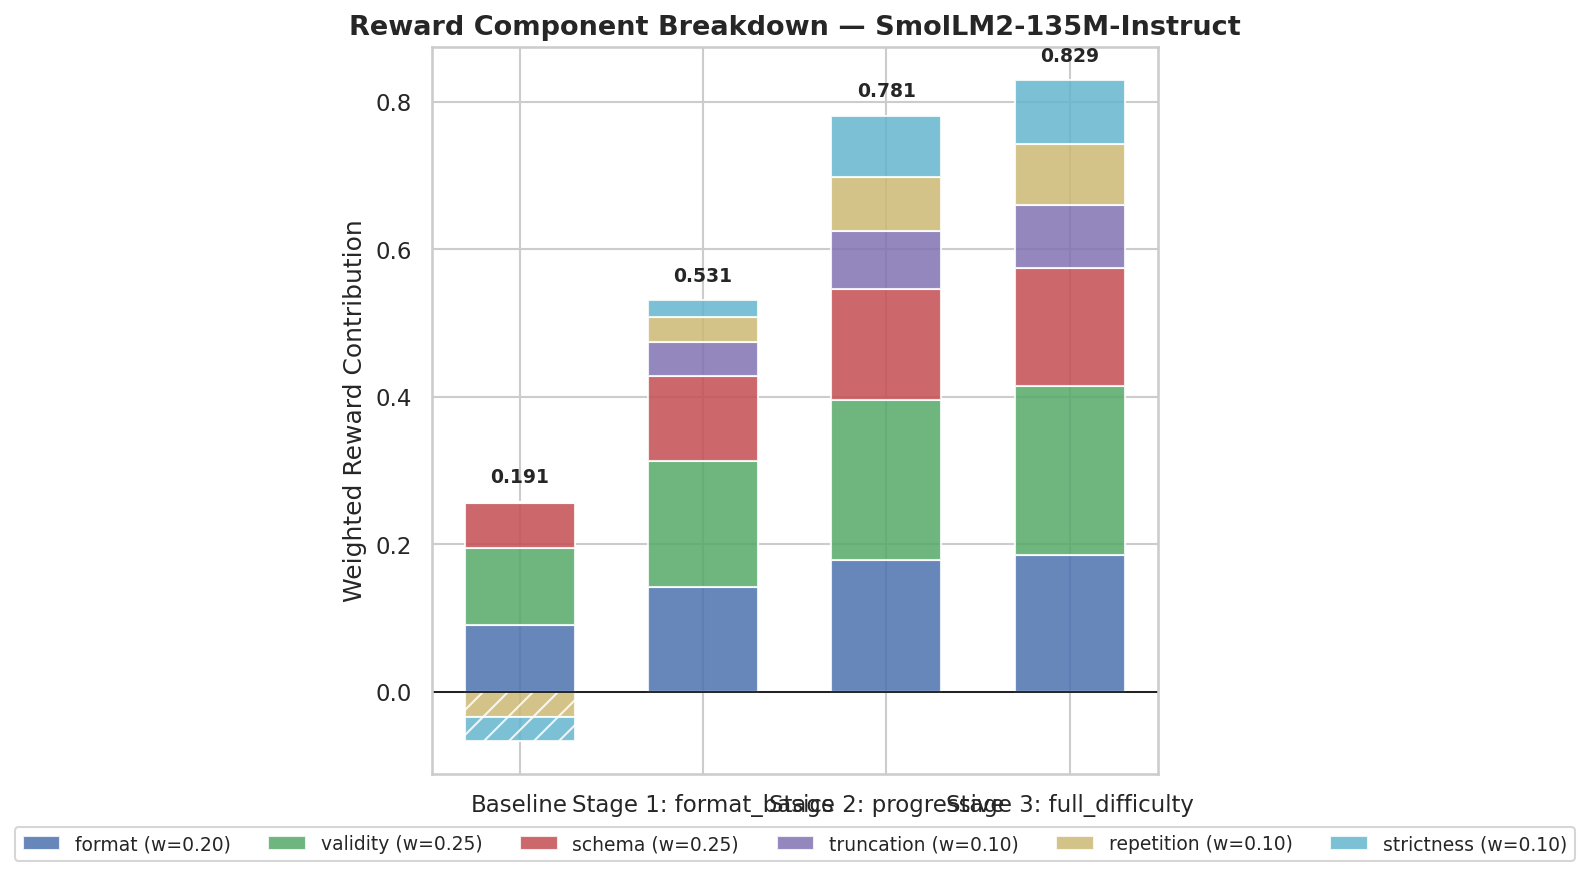
\includegraphics[width=0.82\linewidth]{../../experiments/logs/grpo/nothink/curriculum/smollm2-135m/eval_20260410_060558/figures/reward_breakdown.png}
  \\[0.4em]
  \small No-Think / Curriculum — component contributions at final checkpoint
\end{frame}

% ── Slide 6 · Training Strategies ──────────────────────
\begin{frame}{Training Strategies}
  \begin{columns}[T]
    \begin{column}{0.44\textwidth}
      \renewcommand{\arraystretch}{1.5}
      \begin{tabular}{@{}lcc@{}}
        \toprule
                          & \textbf{Standard} & \textbf{Curriculum} \\
        \midrule
        \textbf{No-Think} & $\checkmark$      & $\checkmark$ \\
        \textbf{Think}    & $\checkmark$      & $\checkmark$ \\
        \bottomrule
      \end{tabular}
      \vspace{0.7em}\\
      \small
      \textbf{Think:} model generates \texttt{<think>} reasoning before JSON\\[0.4em]
      \textbf{Curriculum:} 3 progressive stages
    \end{column}
    \begin{column}{0.53\textwidth}
      \small
      \renewcommand{\arraystretch}{1.35}
      \begin{tabular}{@{}lrcc@{}}
        \toprule
        \textbf{Stage}       & \textbf{Steps} & \textbf{S\,/\,M\,/\,H} & \textbf{Temp} \\
        \midrule
        1 – Format Basics    & 800  & 35\,/\,55\,/\,10\%  & 0.8 \\
        2 – Progressive      & 800  & 15\,/\,35\,/\,50\%  & 0.7 \\
        3 – Full Difficulty  & 900  & 10\,/\,25\,/\,65\%  & 0.6 \\
        \bottomrule
      \end{tabular}
      \vspace{0.3em}\\
      \small S\,=\,Simple\quad M\,=\,Medium\quad H\,=\,Hard
    \end{column}
  \end{columns}
\end{frame}

% ── Slide 7 · Dataset ───────────────────────────────────
\begin{frame}{Parametric Synthetic Dataset}
  \begin{columns}[T]
    \begin{column}{0.48\textwidth}
      \begin{itemize}
        \setlength\itemsep{0.55em}
        \item 24 parameterized templates\\(8 per difficulty tier)
        \item 1\,500 samples/stage $\times$ 3 stages\\
              = \textbf{4\,500} training samples
        \item Eval: \textbf{300 samples} — 100 simple / 100 medium / 100 hard
        \item \textbf{No ground-truth JSON}\\
              reward functions evaluate directly
      \end{itemize}
    \end{column}
    \begin{column}{0.48\textwidth}
      \begin{block}{Difficulty tiers}
        \small
        \textbf{Simple} — flat key-value objects, typed arrays\\[0.4em]
        \textbf{Medium} — nested objects, config files, form schemas\\[0.4em]
        \textbf{Hard} — JSON Schema draft-07, paginated APIs, OpenAPI specs
      \end{block}
    \end{column}
  \end{columns}
\end{frame}

% ════════════════════════════════════════════════════════════
%  NO-THINK · STANDARD
% ════════════════════════════════════════════════════════════

% ── Table 1 · Baseline (No-Think Standard) ───────────────
\begin{frame}{Table 1 — Baseline Pass@1 (No-Think)}
  \centering
  \footnotesize
  \renewcommand{\arraystretch}{1.55}
  \setlength\tabcolsep{10pt}
  \begin{tabular}{@{}lcccc@{}}
    \toprule
    \textbf{Model} & \textbf{Overall} & \textbf{Simple} & \textbf{Medium} & \textbf{Hard} \\
    \midrule
    SmolLM2-135M   & 39.00\% & 58.00\% & 39.00\% & 20.00\% \\
    SmolLM2-360M   & 77.67\% & 85.00\% & 86.00\% & 62.00\% \\
    Qwen2.5-0.5B   & 92.67\% & 95.00\% & 95.00\% & 88.00\% \\
    TinyLlama-1.1B & 79.33\% & 89.00\% & 76.00\% & 73.00\% \\
    Gemma-2-2B     & \textbf{98.33\%} & \textbf{100\%} & \textbf{100\%} & \textbf{95.00\%} \\
    \bottomrule
  \end{tabular}
  \vspace{0.6em}

  \small 300-sample balanced eval set (100 simple / 100 medium / 100 hard)
\end{frame}

% ── Table 2 · Post-training (No-Think Standard) ─────────
\begin{frame}{Table 2 — Post-Training Pass@1 (No-Think / Standard, 2\,500 steps)}
  \centering
  \footnotesize
  \renewcommand{\arraystretch}{1.55}
  \setlength\tabcolsep{7pt}
  \begin{tabular}{@{}lccccc@{}}
    \toprule
    \textbf{Model} & \textbf{Overall} & \textbf{Simple} & \textbf{Medium} & \textbf{Hard} & $\boldsymbol{\Delta}$ \\
    \midrule
    SmolLM2-135M   & 87.67\% & 87.00\% & 89.00\% & 87.00\% & \alert{$+$48.67} \\
    SmolLM2-360M   & 96.67\% & 97.00\% & 97.00\% & 96.00\% & $+$19.00 \\
    Qwen2.5-0.5B   & 97.33\% & 99.00\% & 95.00\% & \textbf{98.00\%} & $+$4.67  \\
    TinyLlama-1.1B & \textbf{97.67\%} & \textbf{100\%} & 96.00\% & 97.00\% & $+$18.33 \\
    Gemma-2-2B     & 96.67\% & \textbf{100\%} & \textbf{99.00\%} & 91.00\% & \alert{$-$1.67} \\
    \bottomrule
  \end{tabular}
  \vspace{0.5em}

  \small Gemma-2-2B regresses ($-$1.67 pp) — mixed-difficulty training without curriculum
\end{frame}

% ── Figure · SmolLM2-135M No-Think / Standard ────────────
\begin{frame}{SmolLM2-135M — Baseline vs.\ GRPO (No-Think / Standard)}
  \centering
  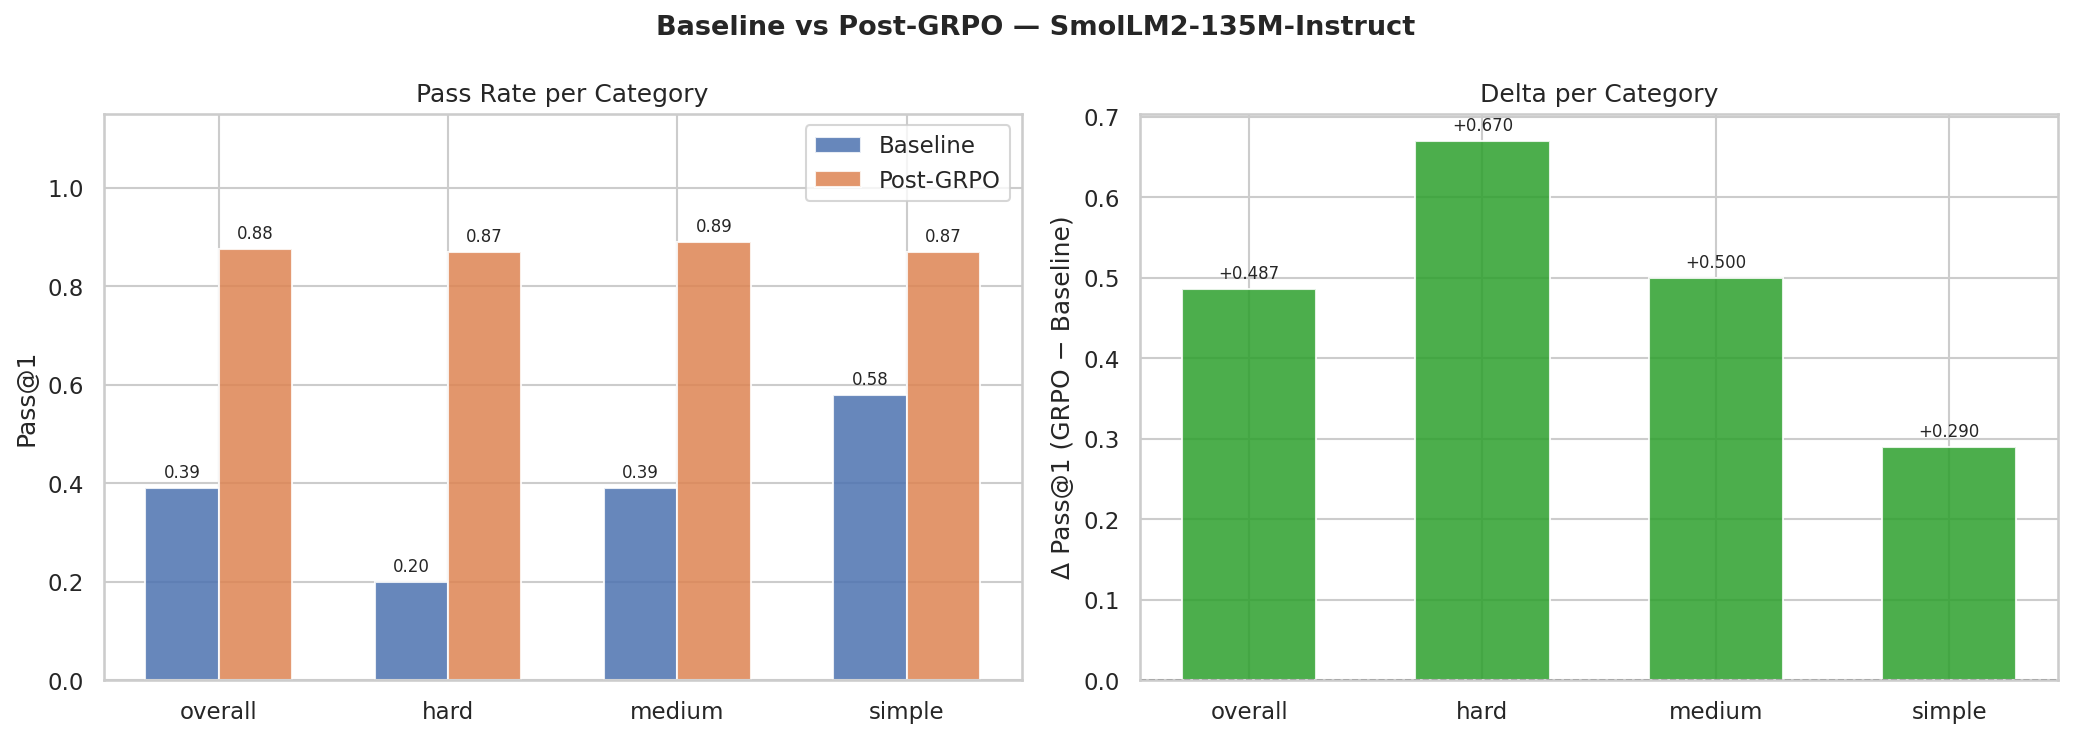
\includegraphics[width=0.78\linewidth]{../../experiments/logs/grpo/nothink/standard/smollm2-135m/eval_20260409_152243/figures/baseline_vs_grpo_comparison.png}
  \\[0.4em]
  \small Pass@1 by difficulty tier before and after 2\,500 GRPO steps
\end{frame}

% ════════════════════════════════════════════════════════════
%  NO-THINK · CURRICULUM
% ════════════════════════════════════════════════════════════

% ── Table 3 · Baseline (No-Think Curriculum) ─────────────
\begin{frame}{Table 3 — Baseline Pass@1 (No-Think / Curriculum)}
  \centering
  \footnotesize
  \renewcommand{\arraystretch}{1.55}
  \setlength\tabcolsep{10pt}
  \begin{tabular}{@{}lcccc@{}}
    \toprule
    \textbf{Model} & \textbf{Overall} & \textbf{Simple} & \textbf{Medium} & \textbf{Hard} \\
    \midrule
    SmolLM2-135M   & 33.00\% & 49.00\% & 32.00\% & 18.00\% \\
    SmolLM2-360M   & 73.67\% & 82.00\% & 84.00\% & 55.00\% \\
    Qwen2.5-0.5B   & 89.33\% & \textbf{98.00\%} & 91.00\% & 79.00\% \\
    TinyLlama-1.1B & 79.33\% & 89.00\% & 83.00\% & 66.00\% \\
    Gemma-2-2B     & \textbf{97.00\%} & \textbf{100\%} & \textbf{98.00\%} & \textbf{93.00\%} \\
    \bottomrule
  \end{tabular}
  \vspace{0.6em}

  \small Slight variance vs.\ Table 1 due to different generation seed
\end{frame}

% ── Table 4 · Post-training (No-Think Curriculum) ────────
\begin{frame}{Table 4 — Post-Training Pass@1 (No-Think / Curriculum, 2\,500 steps)}
  \centering
  \footnotesize
  \renewcommand{\arraystretch}{1.55}
  \setlength\tabcolsep{7pt}
  \begin{tabular}{@{}lccccc@{}}
    \toprule
    \textbf{Model} & \textbf{Overall} & \textbf{Simple} & \textbf{Medium} & \textbf{Hard} & $\boldsymbol{\Delta}$ \\
    \midrule
    SmolLM2-135M   & 89.00\% & 90.00\% & 86.00\% & 91.00\% & \alert{$+$56.00} \\
    SmolLM2-360M   & 95.33\% & 93.00\% & 95.00\% & \textbf{98.00\%} & $+$21.67 \\
    Qwen2.5-0.5B   & 97.33\% & \textbf{100\%} & 95.00\% & 97.00\% & $+$8.00  \\
    TinyLlama-1.1B & \textbf{99.33\%} & \textbf{100\%} & \textbf{99.00\%} & \textbf{99.00\%} & $+$20.00 \\
    Gemma-2-2B     & 97.67\% & \textbf{100\%} & \textbf{99.00\%} & 94.00\% & $+$0.67  \\
    \bottomrule
  \end{tabular}
  \vspace{0.5em}

  \small Curriculum protects Gemma-2-2B from regression ($+$0.67 vs.\ $-$1.67 in standard)
\end{frame}

% ── Table 5 · Curriculum Stages (No-Think) ───────────────
\begin{frame}{Table 5 — Curriculum Stage Progression (No-Think)}
  \centering
  \footnotesize
  \renewcommand{\arraystretch}{1.55}
  \setlength\tabcolsep{9pt}
  \begin{tabular}{@{}lcccc@{}}
    \toprule
    \textbf{Model} & \textbf{Baseline} & \textbf{Stage 1} & \textbf{Stage 2} & \textbf{Stage 3} \\
    \midrule
    SmolLM2-135M   & 33.00\% & 62.67\% & 84.67\% & \textbf{89.00\%} \\
    SmolLM2-360M   & 73.67\% & 79.67\% & 91.33\% & \textbf{95.33\%} \\
    Qwen2.5-0.5B   & 89.33\% & 95.67\% & 97.00\% & \textbf{97.33\%} \\
    TinyLlama-1.1B & 79.33\% & 94.33\% & 98.33\% & \textbf{99.33\%} \\
    Gemma-2-2B     & \textbf{97.00\%} & \textbf{98.33\%} & 97.67\% & 97.67\% \\
    \bottomrule
  \end{tabular}
  \vspace{0.5em}

  \small Monotonic improvement for all models; Gemma peaks at Stage 1
\end{frame}

% ── Figure · SmolLM2-135M No-Think / Curriculum ──────────
\begin{frame}{SmolLM2-135M — Curriculum Progression (No-Think)}
  \centering
  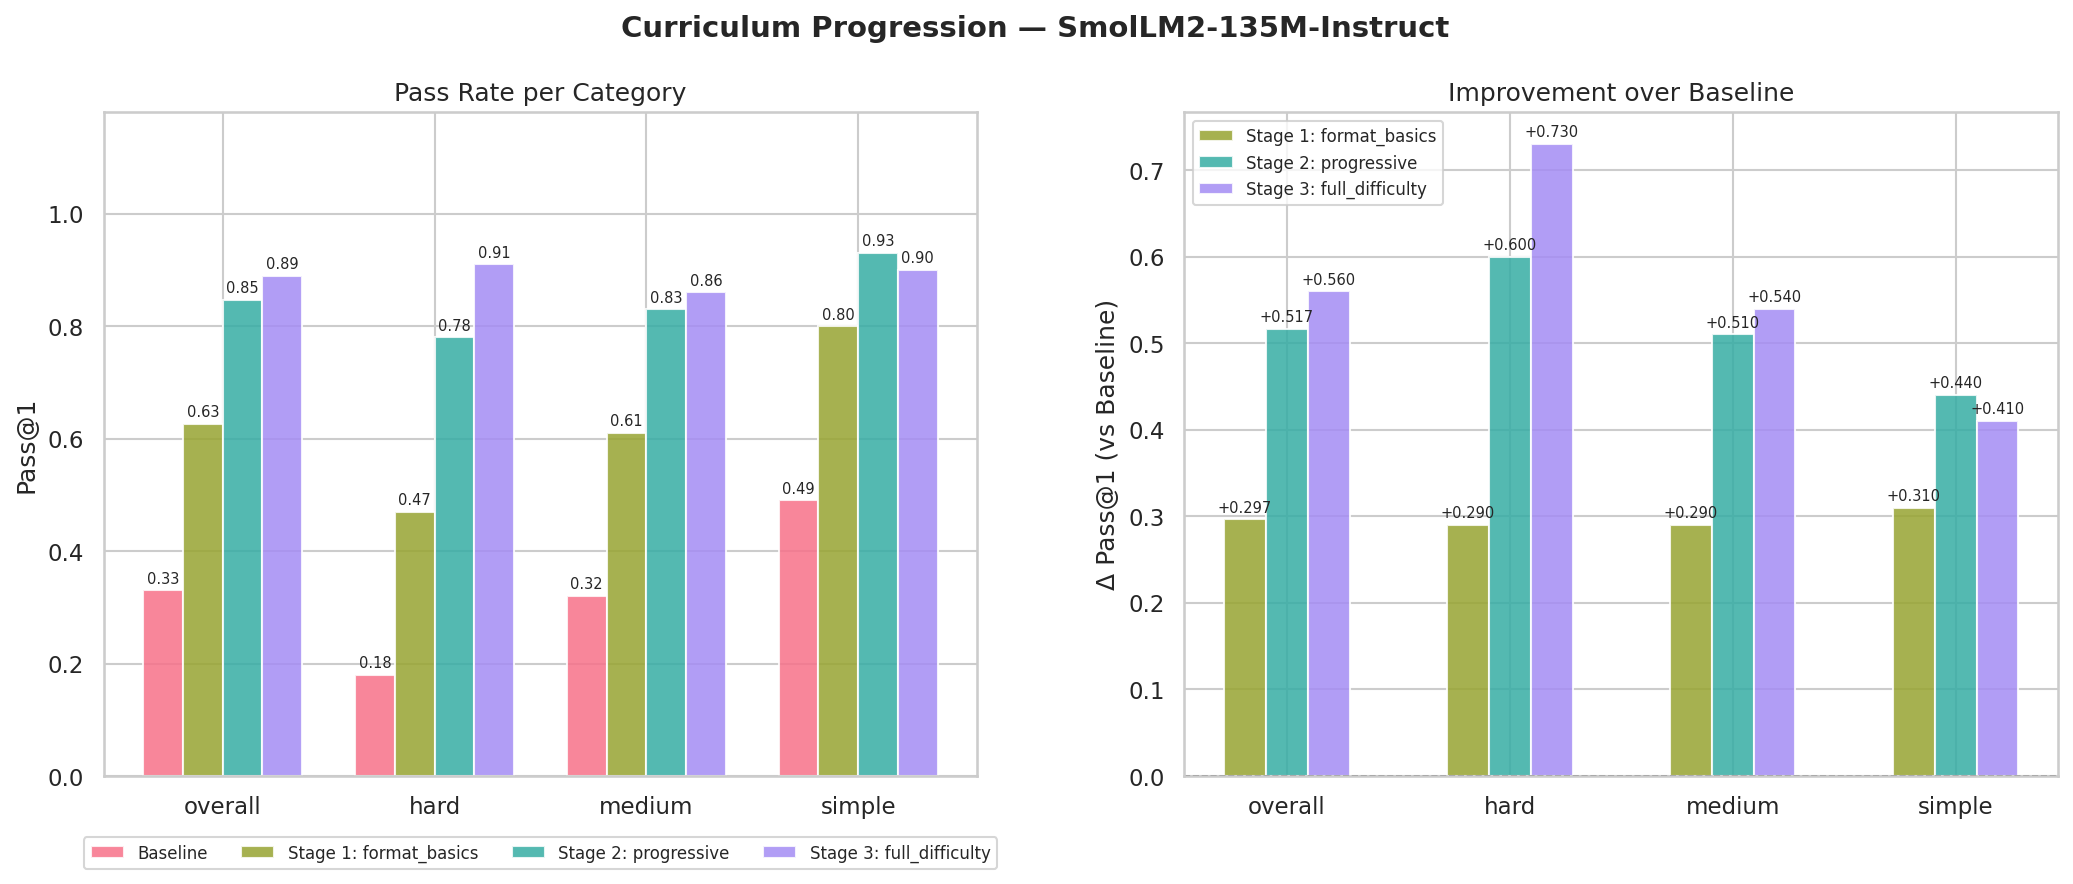
\includegraphics[width=0.78\linewidth]{../../experiments/logs/grpo/nothink/curriculum/smollm2-135m/eval_20260410_060558/figures/curriculum_progression.png}
  \\[0.4em]
  \small 33\% $\to$ 62.7\% $\to$ 84.7\% $\to$ 89.0\% across 3 curriculum stages
\end{frame}

% ── Heatmap · SmolLM2-135M No-Think / Curriculum ─────────
\begin{frame}{SmolLM2-135M — Difficulty Heatmap (No-Think / Curriculum)}
  \centering
  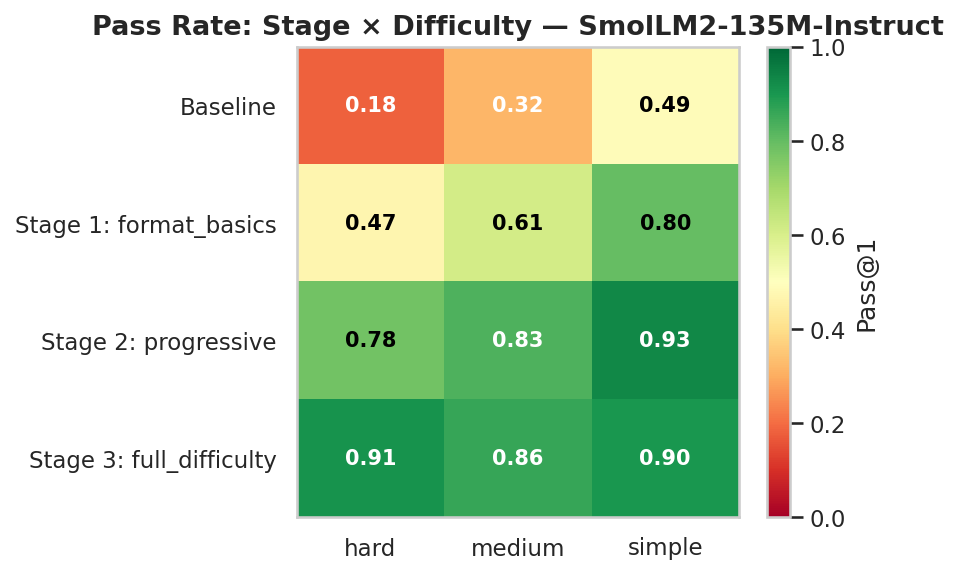
\includegraphics[width=0.78\linewidth]{../../experiments/logs/grpo/nothink/curriculum/smollm2-135m/eval_20260410_060558/figures/stage_difficulty_heatmap.png}
  \\[0.4em]
  \small Pass@1 per difficulty tier at each curriculum stage
\end{frame}

% ════════════════════════════════════════════════════════════
%  THINK · STANDARD
% ════════════════════════════════════════════════════════════

% ── Table 6 · Baseline (Think Standard) ──────────────────
\begin{frame}{Table 6 — Baseline Pass@1 (Think)}
  \centering
  \footnotesize
  \renewcommand{\arraystretch}{1.55}
  \setlength\tabcolsep{10pt}
  \begin{tabular}{@{}lcccc@{}}
    \toprule
    \textbf{Model} & \textbf{Overall} & \textbf{Simple} & \textbf{Medium} & \textbf{Hard} \\
    \midrule
    SmolLM2-135M   & 31.33\% & 44.00\% & 33.00\% & 17.00\% \\
    SmolLM2-360M   & 69.33\% & 79.00\% & 80.00\% & 49.00\% \\
    Qwen2.5-0.5B   & 90.33\% & \textbf{98.00\%} & 92.00\% & 81.00\% \\
    TinyLlama-1.1B & 85.67\% & 90.00\% & 87.00\% & 80.00\% \\
    Gemma-2-2B     & \textbf{96.67\%} & 99.00\% & \textbf{98.00\%} & \textbf{93.00\%} \\
    \bottomrule
  \end{tabular}
  \vspace{0.6em}

  \small \texttt{<think>} prompt lowers baseline for small models (360M: 77.67\% $\to$ 69.33\%)
\end{frame}

% ── Table 7 · Post-training (Think Standard) ─────────────
\begin{frame}{Table 7 — Post-Training Pass@1 (Think / Standard, 2\,500 steps)}
  \centering
  \footnotesize
  \renewcommand{\arraystretch}{1.55}
  \setlength\tabcolsep{7pt}
  \begin{tabular}{@{}lccccc@{}}
    \toprule
    \textbf{Model} & \textbf{Overall} & \textbf{Simple} & \textbf{Medium} & \textbf{Hard} & $\boldsymbol{\Delta}$ \\
    \midrule
    SmolLM2-135M   & 90.00\% & 96.00\% & 87.00\% & 87.00\% & \alert{$+$58.67} \\
    SmolLM2-360M   & 95.67\% & 96.00\% & 97.00\% & 94.00\% & $+$26.33 \\
    Qwen2.5-0.5B   & 97.67\% & \textbf{100\%} & \textbf{98.00\%} & 95.00\% & $+$7.33  \\
    TinyLlama-1.1B & \textbf{98.67\%} & 99.00\% & \textbf{98.00\%} & \textbf{99.00\%} & $+$13.00 \\
    Gemma-2-2B     & 96.00\% & 99.00\% & \textbf{99.00\%} & 90.00\% & \alert{$-$0.67} \\
    \bottomrule
  \end{tabular}
  \vspace{0.5em}

  \small SmolLM2-135M: largest absolute gain in the study ($+$58.67 pp)
\end{frame}

% ── Figure · SmolLM2-135M Think / Standard ───────────────
\begin{frame}{SmolLM2-135M — Baseline vs.\ GRPO (Think / Standard)}
  \centering
  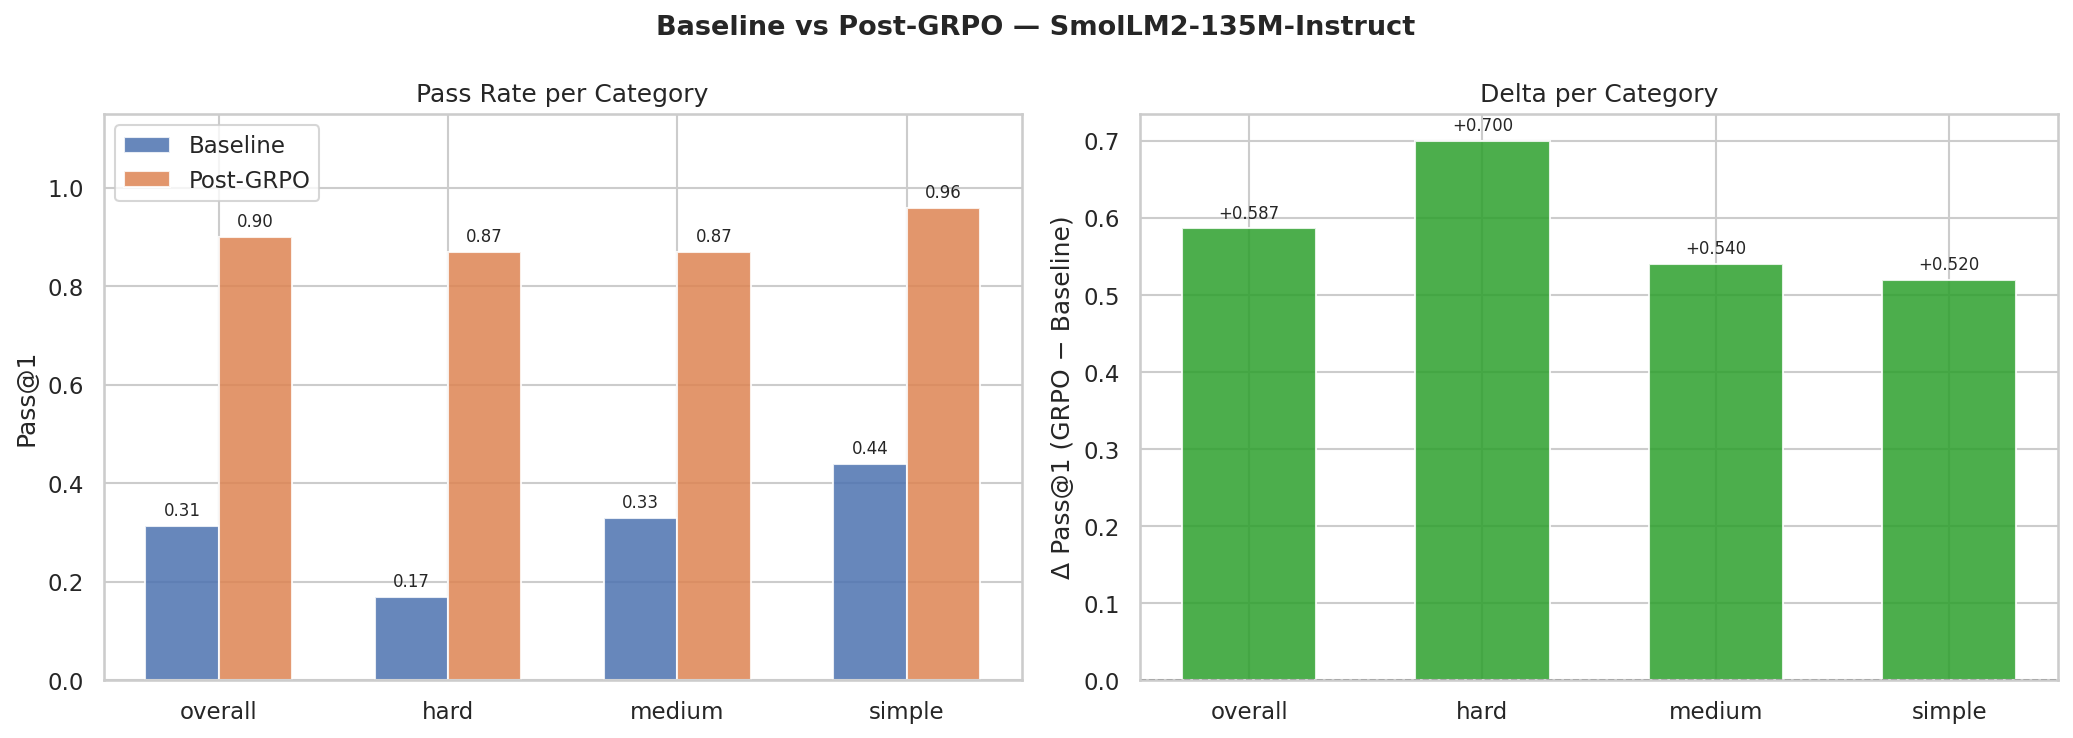
\includegraphics[width=0.78\linewidth]{../../experiments/logs/grpo/think/standard/smollm2-135m/eval_20260411_192610/figures/baseline_vs_grpo_comparison.png}
  \\[0.4em]
  \small Think / Standard — reasoning tokens unlock the highest peak for 135M
\end{frame}

% ════════════════════════════════════════════════════════════
%  THINK · CURRICULUM
% ════════════════════════════════════════════════════════════

% ── Table 8 · Baseline (Think Curriculum) ────────────────
\begin{frame}{Table 8 — Baseline Pass@1 (Think / Curriculum)}
  \centering
  \footnotesize
  \renewcommand{\arraystretch}{1.55}
  \setlength\tabcolsep{10pt}
  \begin{tabular}{@{}lcccc@{}}
    \toprule
    \textbf{Model} & \textbf{Overall} & \textbf{Simple} & \textbf{Medium} & \textbf{Hard} \\
    \midrule
    SmolLM2-135M   & 31.67\% & 51.00\% & 25.00\% & 19.00\% \\
    SmolLM2-360M   & 71.33\% & 76.00\% & 79.00\% & 59.00\% \\
    Qwen2.5-0.5B   & 91.67\% & \textbf{99.00\%} & 89.00\% & 87.00\% \\
    TinyLlama-1.1B & 83.67\% & 96.00\% & 84.00\% & 71.00\% \\
    Gemma-2-2B     & \textbf{96.33\%} & \textbf{100\%} & \textbf{96.00\%} & \textbf{93.00\%} \\
    \bottomrule
  \end{tabular}
  \vspace{0.6em}

  \small Same capability hierarchy as Table 6; slight sampling variance
\end{frame}

% ── Table 9 · Post-training (Think Curriculum) ───────────
\begin{frame}{Table 9 — Post-Training Pass@1 (Think / Curriculum, 2\,500 steps)}
  \centering
  \footnotesize
  \renewcommand{\arraystretch}{1.55}
  \setlength\tabcolsep{7pt}
  \begin{tabular}{@{}lccccc@{}}
    \toprule
    \textbf{Model} & \textbf{Overall} & \textbf{Simple} & \textbf{Medium} & \textbf{Hard} & $\boldsymbol{\Delta}$ \\
    \midrule
    SmolLM2-135M   & 89.33\% & 94.00\% & 88.00\% & 86.00\% & \alert{$+$57.67} \\
    SmolLM2-360M   & 93.00\% & 92.00\% & 97.00\% & 90.00\% & $+$21.67 \\
    Qwen2.5-0.5B   & \textbf{98.00\%} & \textbf{100\%} & \textbf{97.00\%} & \textbf{97.00\%} & $+$6.33  \\
    TinyLlama-1.1B & 97.67\% & \textbf{100\%} & 96.00\% & \textbf{97.00\%} & $+$14.00 \\
    Gemma-2-2B     & 97.67\% & 99.00\% & \textbf{99.00\%} & 95.00\% & $+$1.33  \\
    \bottomrule
  \end{tabular}
  \vspace{0.5em}

  \small Curriculum fixes Gemma-2-2B: $+$1.33 pp vs.\ $-$0.67 in standard
\end{frame}

% ── Table 10 · Curriculum Stages (Think) ─────────────────
\begin{frame}{Table 10 — Curriculum Stage Progression (Think)}
  \centering
  \footnotesize
  \renewcommand{\arraystretch}{1.55}
  \setlength\tabcolsep{9pt}
  \begin{tabular}{@{}lcccc@{}}
    \toprule
    \textbf{Model} & \textbf{Baseline} & \textbf{Stage 1} & \textbf{Stage 2} & \textbf{Stage 3} \\
    \midrule
    SmolLM2-135M   & 31.67\% & 55.67\% & 80.00\% & \textbf{89.33\%} \\
    SmolLM2-360M   & 71.33\% & 78.33\% & 90.33\% & \textbf{93.00\%} \\
    Qwen2.5-0.5B   & 91.67\% & 94.67\% & 93.33\% & \textbf{98.00\%} \\
    TinyLlama-1.1B & 83.67\% & 94.33\% & \textbf{97.00\%} & 97.67\% \\
    Gemma-2-2B     & \textbf{96.33\%} & 83.00\% & 66.00\% & 97.67\% \\
    \bottomrule
  \end{tabular}
  \vspace{0.5em}

  \small \alert{Gemma-2-2B U-curve}: 96\% $\to$ 83\% $\to$ 66\% $\to$ 98\% — temporary collapse
\end{frame}

% ── Figure · SmolLM2-135M Think / Curriculum ─────────────
\begin{frame}{SmolLM2-135M — Curriculum Progression (Think)}
  \centering
  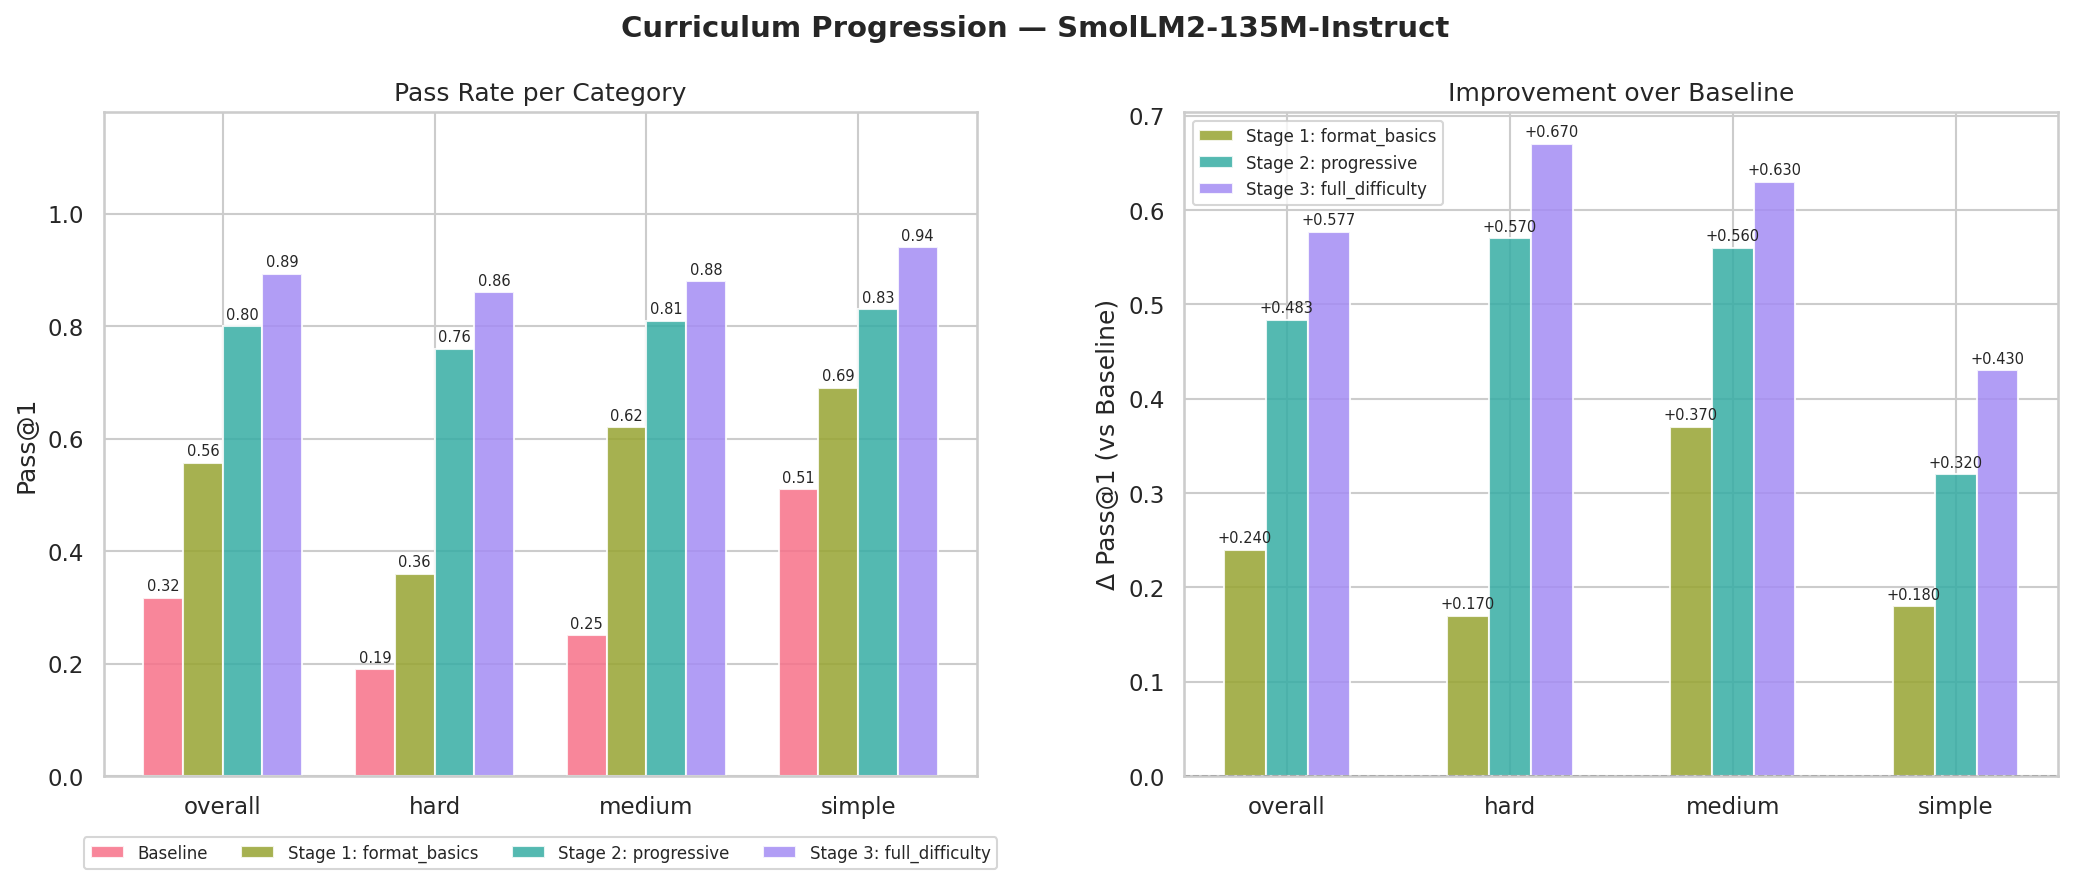
\includegraphics[width=0.78\linewidth]{../../experiments/logs/grpo/think/curriculum/smollm2-135m/eval_20260413_034728/figures/curriculum_progression.png}
  \\[0.4em]
  \small 31.7\% $\to$ 55.7\% $\to$ 80.0\% $\to$ 89.3\% across 3 curriculum stages
\end{frame}

% ── Heatmap · SmolLM2-135M Think / Curriculum ────────────
\begin{frame}{SmolLM2-135M — Difficulty Heatmap (Think / Curriculum)}
  \centering
  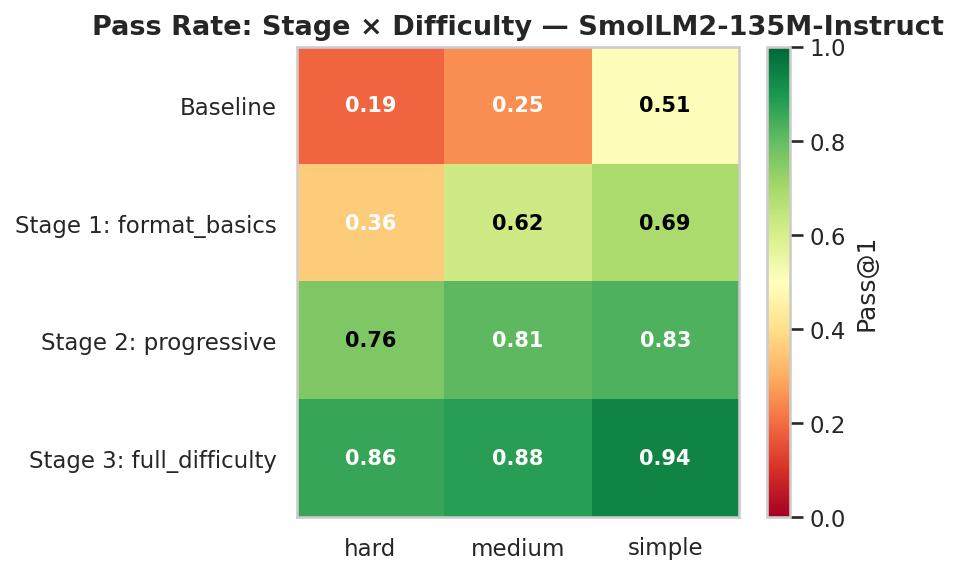
\includegraphics[width=0.78\linewidth]{../../experiments/logs/grpo/think/curriculum/smollm2-135m/eval_20260413_034728/figures/stage_difficulty_heatmap.png}
  \\[0.4em]
  \small Pass@1 per difficulty tier at each curriculum stage
\end{frame}

% ════════════════════════════════════════════════════════════
%  CLOSING
% ════════════════════════════════════════════════════════════

% ── Lessons & Limitations ────────────────────────────────
\begin{frame}{Lessons \& Limitations}
  \begin{columns}[T]
    \begin{column}{0.52\textwidth}
      \textbf{Technical lessons}
      \begin{itemize}
        \setlength\itemsep{0.5em}
        \item \textbf{Additive rewards $>$ gating}\\*
              zero-advantage collapse if all completions\\* tie $\to$ gradient vanishes
        \item \textbf{Graduated partial credit} matters\\*
              binary validity $\to$ no signal for near-valid JSON
        \item \textbf{4-bit NF4 + LoRA} ($r{=}16$) is sufficient\\*
              $<$2\% of parameters trained, single GPU
        \item \textbf{Weight redistribution} when Think is off\\*
              preserves component ratios automatically
      \end{itemize}
    \end{column}
    \begin{column}{0.44\textwidth}
      \textbf{Limitations}
      \begin{itemize}
        \setlength\itemsep{0.5em}
        \item JSON only — not directly\\*
              generalizable to other formats
        \item Fully synthetic dataset\\*
              $\rightarrow$ potential real-world gap
        \item 2\,500 steps / single GPU\\*
              longer runs may yield more
      \end{itemize}
    \end{column}
  \end{columns}
\end{frame}

% ── Conclusions ──────────────────────────────────────────
\begin{frame}{Conclusions}
  \begin{itemize}
    \setlength\itemsep{0.65em}
    \item GRPO $+$ rule-based rewards brings all 5 models to
          \alert{87–99\% Pass@1} — closing the gap to much larger models
    \item \textbf{Standard training} is optimal for weak models:\\*
          SmolLM2-135M $+$48.67 pp, TinyLlama-1.1B $+$18.33 pp
    \item \textbf{Curriculum} is a safety net for strong models:\\*
          Gemma-2-2B flips from $-$1.67 pp (standard) to $+$0.67 pp
    \item \textbf{Think mode} yields $<$2 pp marginal gain —
          extra latency not justified for sub-1B models
    \item All configurations benefit from \textbf{identical hyperparameters},
          confirming that reward design matters more than tuning
  \end{itemize}
\end{frame}

\end{document}
